% !TEX root = ../main.tex
\subsection{Acceptance Correction Results}
\label{14.20::acceptance_correction_results}
% --+ Acceptance correction results for e- +------------------------------------
    DC and FMT acceptances were obtained by following the procedure described in Section \ref{13.13::acceptance_correction}.
    First, we'll study the $Q^2$ and $\nu$ acceptances for the scattered $e^-$.
    $Q^2$ and $\nu$ acceptances are presented in Figures \textbf{TODO} and \textbf{TODO}, respectively.
    Each one is presented in integrated kinematical region for the other variable.

    % TODO. Talk about resulting plots, check if everything is as expected.

% --+ Acceptance correction results for pi+ & pi- +-----------------------------
    Next, we'll look at $z_h$, $P_T^2$, and $\phi_{PQ}$ acceptances for $\pi^+$ and $\pi^-$.
    We can see $z_h$ acceptance in Figure \textbf{TODO}, where... (TODO).

    Next, $P_T^2$ acceptance is presented in Figure \textbf{TODO}, where we see that... (TODO).

    Finally, $\phi_{PQ}$ acceptance is studied in Figure \textbf{TODO}.
    Here, we see... (TODO).

% --+ Plots +-------------------------------------------------------------------
    % \begin{figure}[hbtp]
    %     % Q2.
    %     \begin{subfigure}{.5\textwidth}
    %         \centering
    %         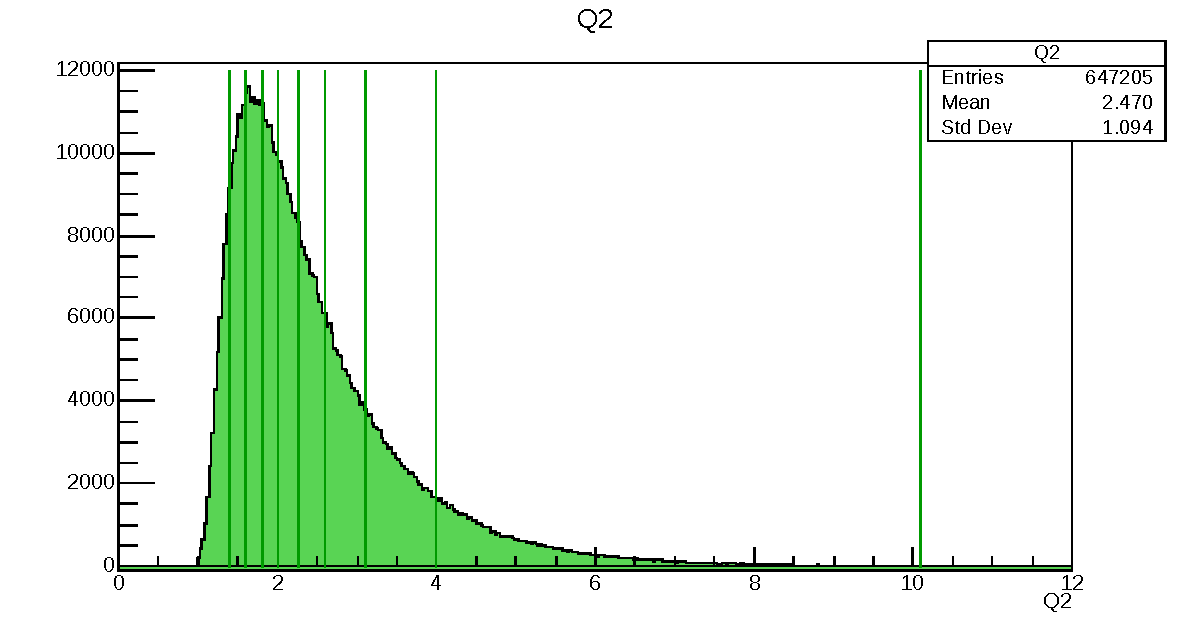
\includegraphics[width=\linewidth]{13dataanalysis/img/40_accbins_q2.pdf}
    %         % \caption{$Q^2$ bins.}
    %         \label{fig::acc_corr_bins_q2}
    %     \end{subfigure}
    %     \begin{subfigure}{.5\textwidth}
    %         \centering
    %         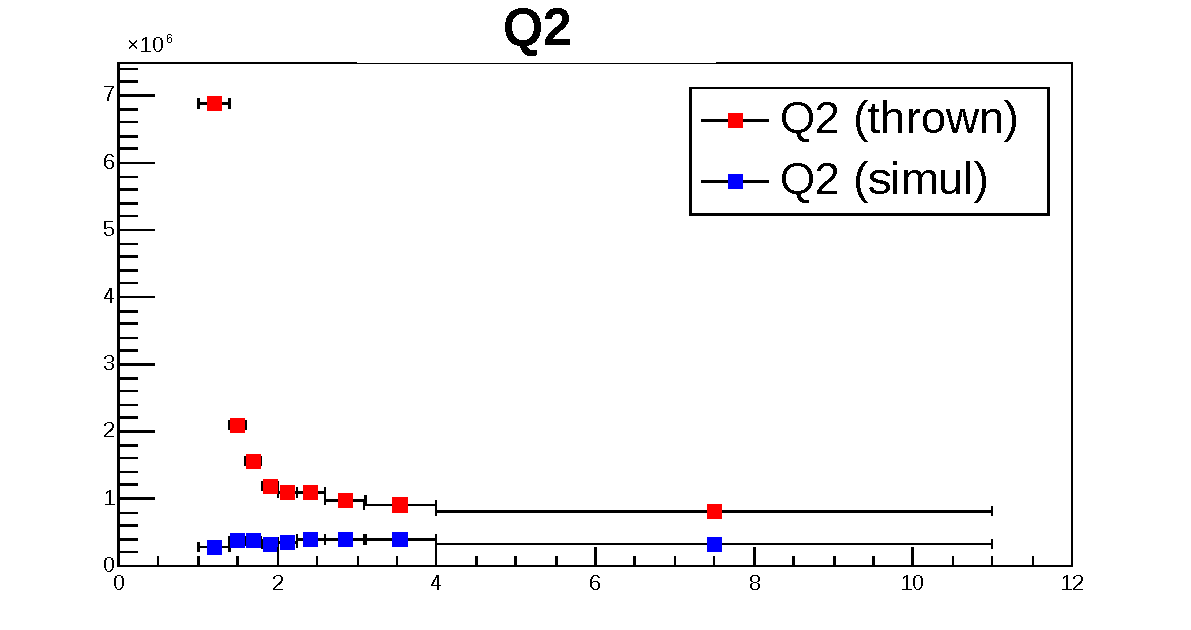
\includegraphics[width=\linewidth]{13dataanalysis/img/40_acccorr_q2.pdf}
    %         % \caption{$Q^2$ acceptance correction results.}
    %         \label{fig::acc_corr_q2}
    %     \end{subfigure}
    %
    %     % nu.
    %     \begin{subfigure}{.5\textwidth}
    %         \centering
    %         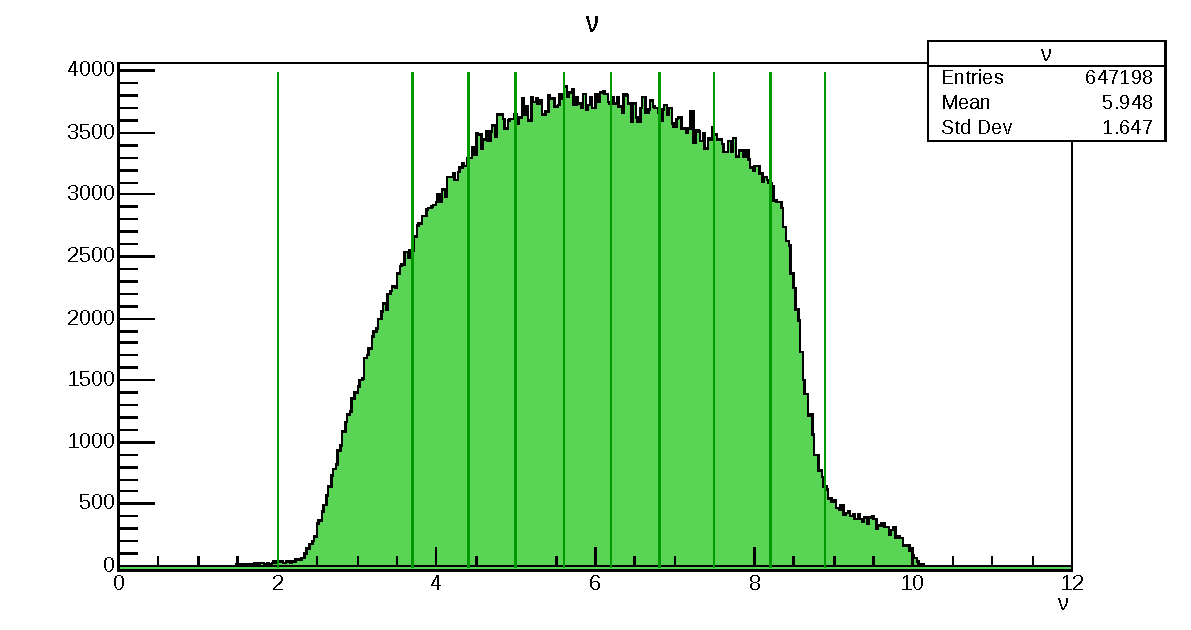
\includegraphics[width=\linewidth]{13dataanalysis/img/40_accbins_nu.pdf}
    %         % \caption{$\nu$ bins.}
    %         \label{fig::acc_corr_bins_nu}
    %     \end{subfigure}
    %     \begin{subfigure}{.5\textwidth}
    %         \centering
    %         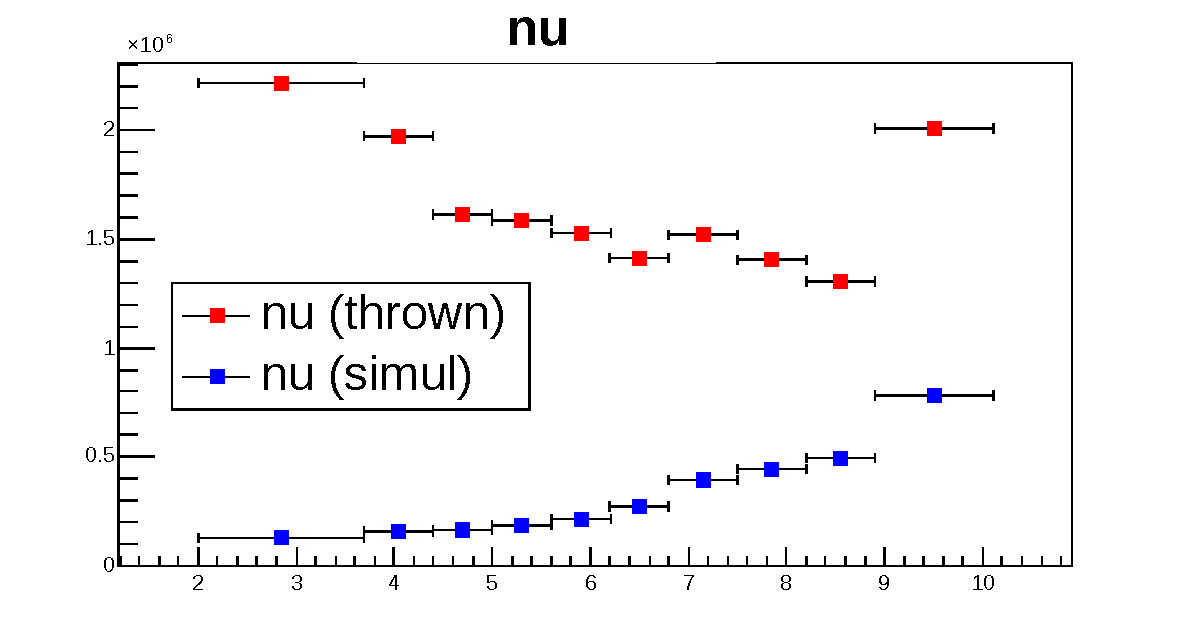
\includegraphics[width=\linewidth]{13dataanalysis/img/40_acccorr_nu.pdf}
    %         % \caption{$\nu$ acceptance correction results.}
    %         \label{fig::acc_corr_nu}
    %     \end{subfigure}
    %
    %     % zh.
    %     \begin{subfigure}{.5\textwidth}
    %         \centering
    %         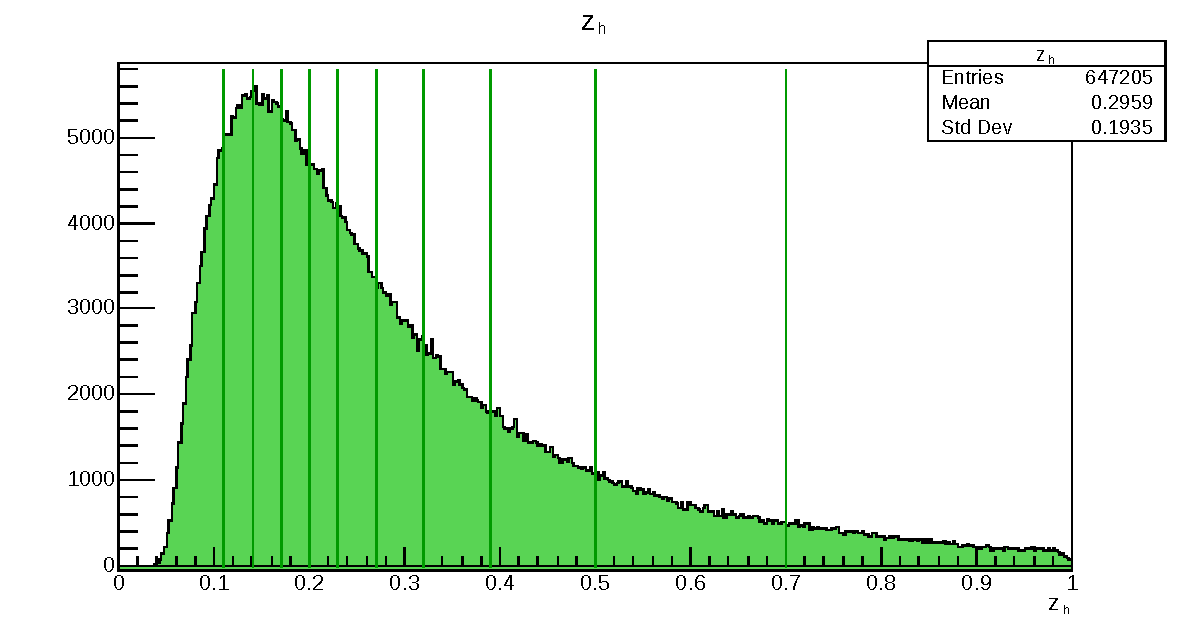
\includegraphics[width=\linewidth]{13dataanalysis/img/40_accbins_zh.pdf}
    %         % \caption{$z_h$ bins.}
    %         \label{fig::acc_corr_bins_zh}
    %     \end{subfigure}
    %     \begin{subfigure}{.5\textwidth}
    %         \centering
    %         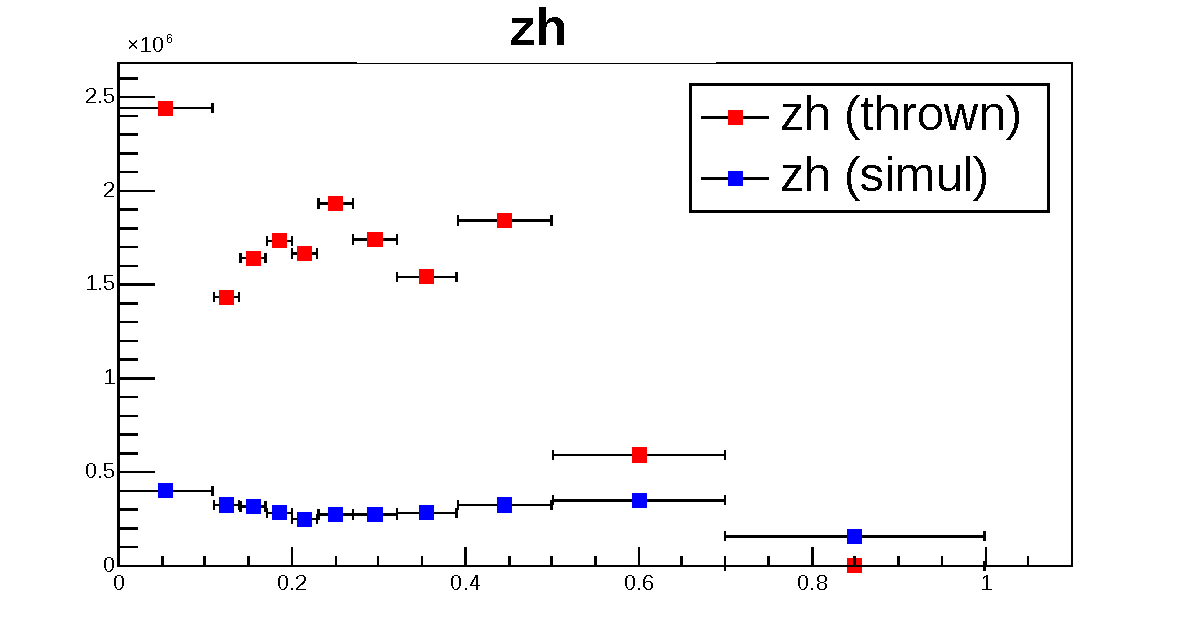
\includegraphics[width=\linewidth]{13dataanalysis/img/40_acccorr_zh.pdf}
    %         % \caption{$z_h$ acceptance correction results.}
    %         \label{fig::acc_corr_zh}
    %     \end{subfigure}
    %
    %     % PT2.
    %     \begin{subfigure}{.5\textwidth}
    %         \centering
    %         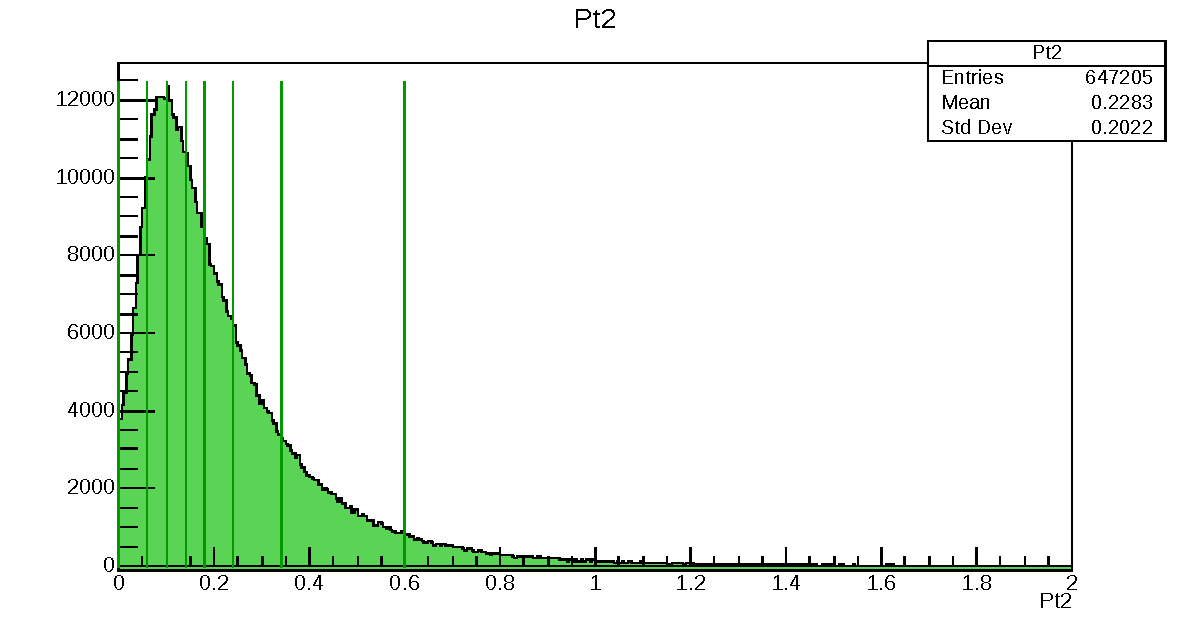
\includegraphics[width=\linewidth]{13dataanalysis/img/40_accbins_pt2.pdf}
    %         % \caption{$P_T^2$ bins.}
    %         \label{fig::acc_corr_bins_pt2}
    %     \end{subfigure}
    %     \begin{subfigure}{.5\textwidth}
    %         \centering
    %         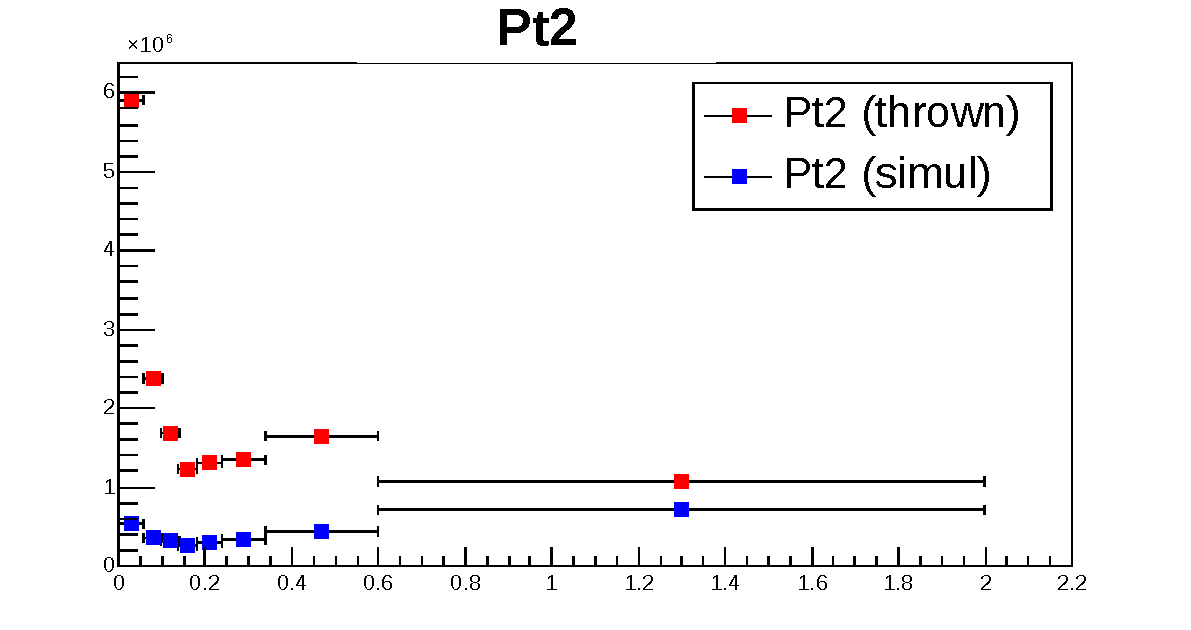
\includegraphics[width=\linewidth]{13dataanalysis/img/40_acccorr_pt2.pdf}
    %         % \caption{$P_T^2$ acceptance correction results.}
    %         \label{fig::acc_corr_pt2}
    %     \end{subfigure}
    %
    %     % phi_PQ.
    %     \begin{subfigure}{.5\textwidth}
    %         \centering
    %         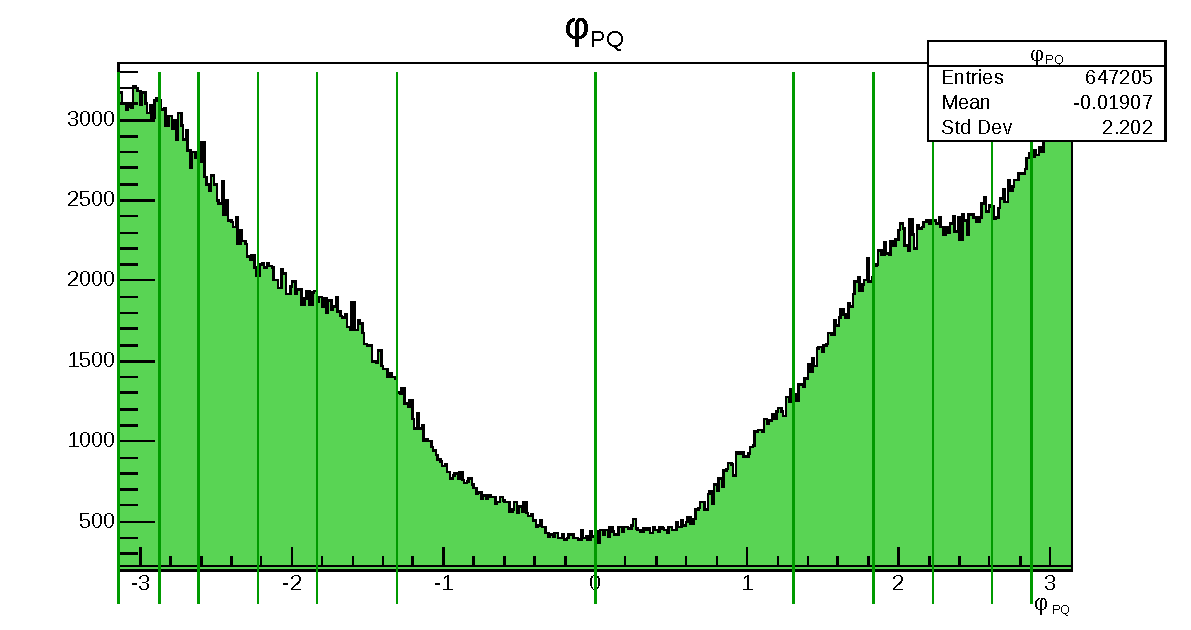
\includegraphics[width=\linewidth]{13dataanalysis/img/40_accbins_phipq.pdf}
    %         % \caption{$\phi_{PQ}$ bins.}
    %         \label{fig::acc_corr_bins_phipq}
    %     \end{subfigure}
    %     \begin{subfigure}{.5\textwidth}
    %         \centering
    %         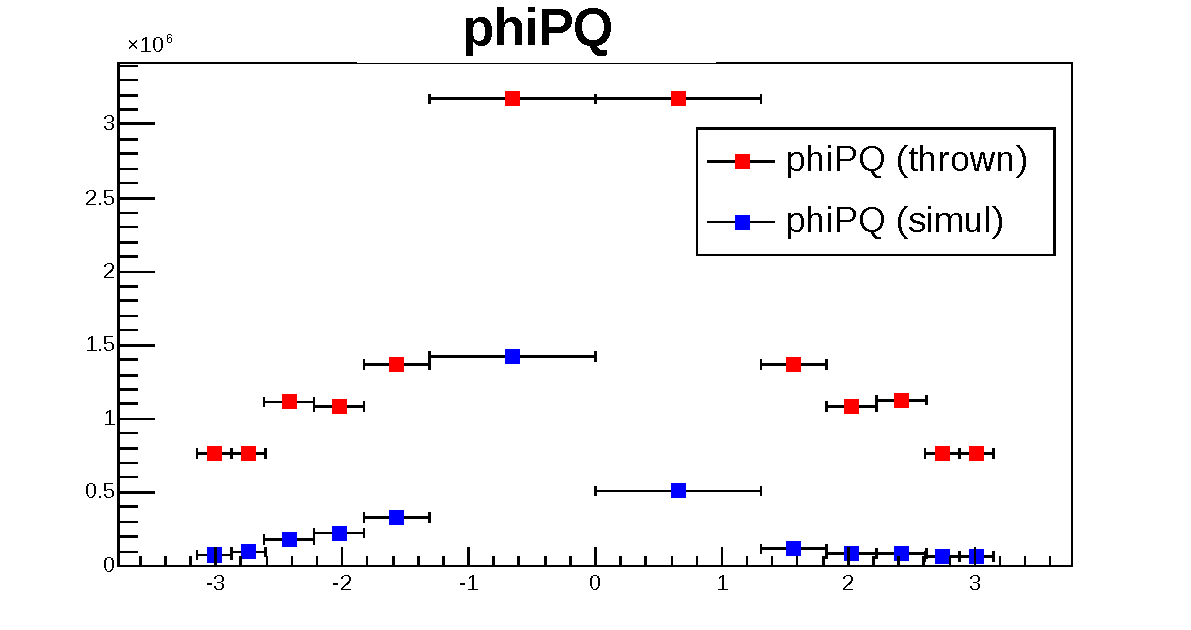
\includegraphics[width=\linewidth]{13dataanalysis/img/40_acccorr_phipq.pdf}
    %         % \caption{$\phi_{PQ}$ acceptance correction results.}
    %         \label{fig::acc_corr_phipq}
    %     \end{subfigure}
    %
    %     \caption[Acceptance correction results.]{Acceptance correction results for the kinematical variables $Q^2$, $\nu$, $z_h$, $p_T^2$, and $\phi_{PQ}$. On the left plots, the acceptance correction bin edges are shown. On the right, the number of thrown (in red) and simulated (in blue) entries for each of the variables is shown. All other variables are integrated for each plot.}
    %     \label{fig::acc_corr}
    % \end{figure}
